\Chapter{Szürkeárnyalatos képek kiszínezése}

A szürkeárnyalatos kép és a megkapott címke térkép segítségével már az előző fejezetben ki tudtuk színezni a szegmenseket, viszont a kiszínezés az eredeti kép árnyalatait nem vette figyelembe. A fejezet célja, hogy a színezést úgy valósítsuk meg, hogy az eredeti kép árnyalatait is megjelenítjük. A minél jobb eredmény elérésének érdekében az RGB és HSV színterekben is megvizsgáltam a problémát, ezeknek a vizsgálatoknak az eredménye a következő alfejezetekben található.

Maguk a színterek a színek matematikai ábrázolásai, lehetővé teszik a színek reprodukálható geometriai ábrázolását a 2D-3D terekben. A színterek a színmodellek és a leképezési függvények kombinációja, és információt tartalmaznak a kép egyes pixeleinek a színéről. A színes képek szegmentálására használt gyakori színterek az RGB, YIQ, HSV, CIE XYZ. \cite{colorspaces}

\Section{RGB}

Az RGB színterű képekben a kép minden egyes pixelét 3 színnel határozzuk meg:
\begin{itemize}
\item vörös (Red)
\item zöld (Green)
\item kék (Blue)
\end{itemize}
A paraméterek a szín intenzitását határozzák meg, az értékük egy 0-255 közötti egész szám. Ha mindegyik paraméterből a maximális, 255 értéket vesszük akkor a fehér színt, ha mindegyikből a minimális, az az a 0 értéket vesszük, akkor pedig a fekete színt kapjuk meg.  Egyszerűsége miatt a színtér széles körben elterjedt. \cite{colorspaces}

Szürkeárnyalatos képek esetén a 3 paraméter értéke megegyezik, így legtöbb esetben csak 1 értékkel szokták a kép pixeleit jelölni, tehát például szürkeárnyalatos képnél egy fekete színű pixel értéke 0.

Ahhoz, hogy egy szürkeárnyalatos képen színt tudjunk megjeleníteni, először át kell alakítanunk RGB színterűvé. Az átalakítást, hasonlóan az előző fejezetben bemutatott \texttt{color\_image} függvényhez, a \texttt{cv2} csomag \texttt{cvtColor} metódusával fogjuk megtenni.
\begin{python}
colored_image = cv2.cvtColor(resized_image, cv2.COLOR_GRAY2RGB)
\end{python}

Egy adott pixelre a színt a következő képlettel határozom meg:
\begin{align*}
 \text{new\_pixel\_color} & = (R, G, B) \\
 Y & = \text{grayscale\_image}[i][j]\\
 R_{ij} & = Y \cdot R / 255 \\
 G_{ij} & = Y \cdot G / 255 \\
 B_{ij} & = Y \cdot B / 255 \\
 \text{colored\_image}_{ij} & = (R_{ij}, G_{ij}, B_{ij})
\end{align*}
\noindent ahol az $i,j$ a kép adott pixelének az indexe.

A pixeleket a \texttt{numpy} csomag \texttt{multiply} függvényével színezem ki a következő kódrészletben látható módon.

\begin{python}
r, g, b = cv2.split(colored_image)

for i in range(0, k):
    np.multiply(r, colors[i][0]/255, out=r,
                where=label_map==i, casting="unsafe")
    np.multiply(g, colors[i][1]/255, out=g,
                where=label_map==i, casting="unsafe")
    np.multiply(b, colors[i][2]/255, out=b,
                where=label_map==i, casting="unsafe")

colored_image = cv2.merge([r, g, b])
\end{python}

Első lépésként a képet a \texttt{cv2.split} segítségével szétválasztom R, G és B komponensekre. Eredményül 3 tömböt kapok, amik az eredeti pixel adott paraméterét tartalmazzák. Ezeken a tömbökön for ciklus segítségével is végig iterálhatnék, és megadhatnám minden pixelnek az értékét a fentebb említett képlet alapján, viszont a \texttt{numpy} csomag \texttt{multiply} függvénye ezt a szorzást sokkal gyorsabban elvégzi. A klaszterek számán haladok végig, ami tulajdonképpen a címkék értékét jelenti és minden címkére elvégzem a szorzást.

A \texttt{multiply} függvény első 2 paramétereként a szorzás 2 tényezőjét várja. Első elemnek az adott komponens tömböt adom meg, második elemnek pedig a címke által meghatározott szín megfelelő komponensének a 255-tel osztott értékét. A \texttt{colors} tömb megegyezik a már korábban bemutatott \texttt{color\_image} függvényben található azonos nevű tömbbel.

A művelet kimeneti értékének ugyanazt a tömböt adom meg. A szorzásnak megadok egy \texttt{where} feltételt, ahol a címke térkép adott elemét fogja vizsgálni a metódus. Megnézi, hogy az adott címke értéke megegyezik-e az éppen vizsgált címkének az értékével és ha igen, csak akkor végzi el a szorzást, tehát csak akkor színezi ki a pixelt.

Utolsó paraméterként a \texttt{casting} paraméternek unsafe értéket állítok be, ez azt jelenti, hogy a nem egyforma típusú értékek esetén is elvégzi a szorzást a függvény.

A szorzások után már csak össze kell olvasztanom a 3 különálló tömböt. Ez a \texttt{cv2.merge} függvénnyel egyszerűen megtudom valósítani. A színezésre példa az \ref{fig:colorized_rgb}.ábrán látható.

\begin{figure}[h]
\centering
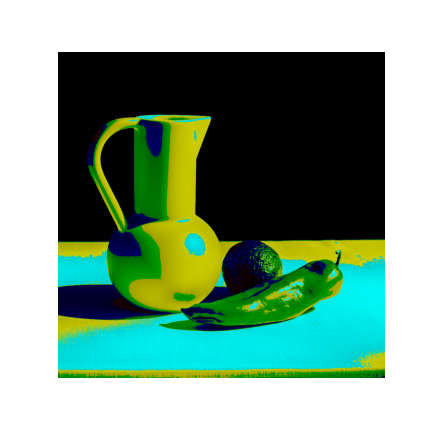
\includegraphics[scale=0.7]{images/colorized_rgb.png}
\caption{Szürkeárnyalatos kép kiszínezése RGB színtérben.}
\label{fig:colorized_rgb}
\end{figure}

Itt már szépen megjelennek az árnyékok, jól kivehetőek a színátmenetek.

\Section{HSV}

A HSV színtér szintén széles körben használt, az emberi szem számára megfelelőbb színtér. A HSV színtérben minden pixelt a következő 3 paraméter határoz meg:
\begin{itemize}
\item színárnyalat (Hue)
\item telítettség (Saturation)
\item érték (Value)
\end{itemize}

A színárnyalat (H) az alapszínt jelöli vagy fokban vagy számokban. A színek skáláját az \ref{tab:hsv_colors}. táblázat szemlélteti.

\begin{table}[h]
\centering
\caption{HSV színtér színárnyalatainak az értéke.}
\label{tab:hsv_colors}
\medskip
\begin{tabular}{|c|c|c|}
\hline
Érték fokban & Érték számmal & Értékhez tartozó szín \\
\hline
0$^{\circ}$ vagy 360$^{\circ}$ & 0 vagy 6 & Vörös \\
\hline
60$^{\circ}$ & 1 & Sárga \\
\hline
120$^{\circ}$ & 2 & Zöld \\
\hline
180$^{\circ}$ & 3 & Cián \\
\hline
240$^{\circ}$ & 4 & Kék \\
\hline
300$^{\circ}$ & 5 & Magenta \\
\hline
\end{tabular}
\end{table}

A telítettség (S) azt írja le, hogy a szín milyen mennyiségben tartalmazza a fehér színt. A telítettséget mindig százalékos értékben adjuk meg, a 100\% jelenti a teljesen telített színt. Minél kisebb az értéke, annál halványabb a szín, mivel egyre több szürkét tartalmaz.

Az értéket (V) szokták fényerőnek (Brightness) is hívni, olyankor a színteret HSB színtérként emlegetik, de ez megegyezik a HSV színtérrel. A az érték a szín sötétségét fejezi ki százalékos arányban, ahol a 0\% a fekete, a 100\% a fehér színt jelenti. \cite{colorspaces}

A HSV színtérben található szürkeárnyalatos képek a H és S csatornákon 0 értékeket tartalmaznak, a kép csak a V értékeiből áll. Ahhoz, hogy szürkeárnyalatosból színes képet tudjunk készíteni, szükségünk van mind a H és mind az S csatorna értékeire. Az \ref{fig:hsv_colorization}. ábra szemlélteti a színezés megvalósításának lehetőségeit.

\begin{figure}[h]
\centering
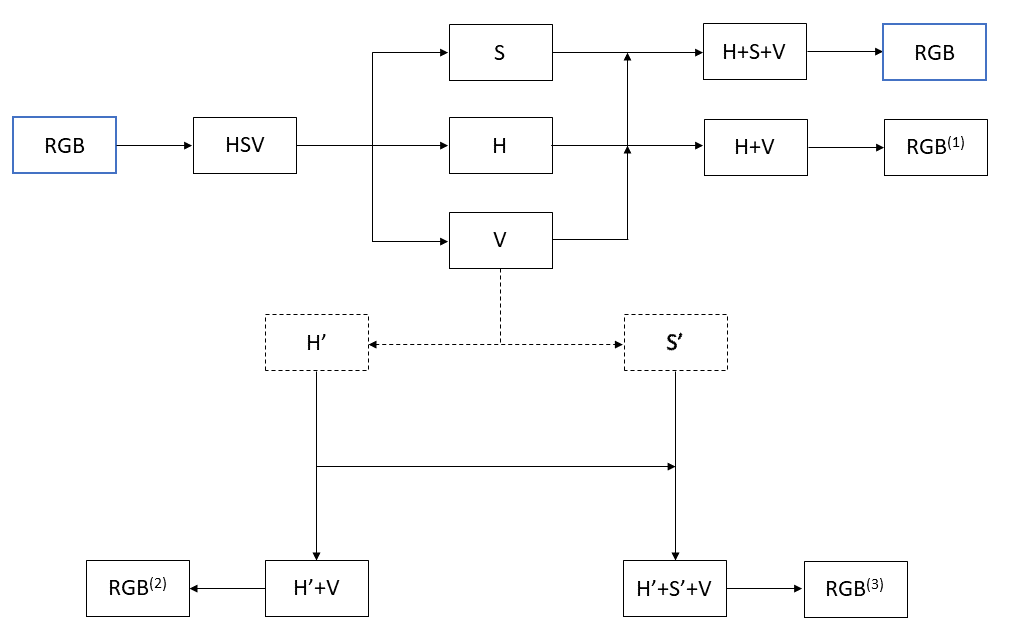
\includegraphics[scale=0.5]{images/hsv_colorization.png}
\caption{Kép színének visszabecslése HSV színtérben.}
\label{fig:hsv_colorization}
\end{figure}

Az ábra abból indul ki hogy van egy RGB színterű képünk, ezt átalakítjuk HSV színterűvé. Ha csatornáira bontjuk a képet, akkor a V  jelzi nekünk a szürkeárnyalatos képet. Amennyiben ismerjük az eredeti H és S csatornákat, akkor jól látható, hogy az eredeti képet fogjuk visszakapni. Amennyiben csak a H értékeit ismerjük, abban az esetben az $RGB^{(1)}$ kép elég hasonló, de színerősségben nagy valószínűséggel különböző lesz. Ezek azok az esetek, amikor valahonnan visszakapjuk ezeket az értékeket, például ha egyébként megvan az eredeti RGB kép és onnan meghatározzuk őket.

Amennyiben csak egy szürkeárnyalatos képünk van, abban az esetben ezeket a csatornákat valahogyan meg kell becsülnünk. Az ábrán a szaggatott vonal jelképezi a becslést, a becsült csatornákat pedig H' és S' jelöli.

Amennyiben a H csatornát tudjuk csak megbecsülni, abban az esetben az S értékének valamilyen átlagértéket veszünk. A kapott $RGB^{(2)}$ képünk nagyban el fog térni az eredeti képtől, hiszen a színek sem biztos hogy pontosak, az árnyalatuk pedig csak egy meghatározott átlag érték, tehát ha az eredeti kép nagyon erős színeket tartalmaz vagy nagyon halvány színeket, akkor az eredmény képünk nagyon eltérő lesz tőle.

Amennyiben viszont az S értékét is vissza tudjuk becsülni, abban az esetben az $RGB^{(3)}$ valószínűleg annyira pontos nem lesz, mintha meglenne az eredeti H és S csatorna, viszont pontosabb lesz mint az $RGB^{(1)}$ illetve az $RGB^{(2)}$.

A \texttt{colors} tömb felhasználásával egyszerűen ki lehet színezni egy szürkeárnyalatos HSV színterű képet. Az RGB színeket átalakítva HSV színterű színekké megkapjuk a H, illetve az S értékét is a színnek. Ezután már csak annyi dolgunk van, hogy ezeket az értékeket átadjuk az összes pixelnek. Egy ilyen színezés megvalósításának a kódja látható a következő kódrészletben.
\begin{python}
import colorsys

colored_image_rgb = cv2.cvtColor(resized_image, cv2.COLOR_GRAY2RGB)

hsv_image = cv2.cvtColor(colored_image_rgb, cv2.COLOR_RGB2HSV)

colored_hsv = hsv_image

for label in range(k):
    color_hsv = colorsys.rgb_to_hsv(
        colors[label][0]/255,
        colors[label][1]/255,
        colors[label][2]/255)
    for i in range(1024):
        for j in range(1024):
            if(label_map[i][j] == label):
                colored_hsv[i][j] =\
                [color_hsv[0]*180, color_hsv[1]*255, hsv_image[i][j][2]]
\end{python}

A színek konvertálására a \texttt{colorsys} csomagot használom, abból is az \texttt{rgb\_to\_hsv} függvényt, ami bemenetként az RGB szín csatornáit várja 0 és 1 közötti értékként, ezért a szín minden értékét el kell osztani 255-tel. A meglévő szürkeárnyalatos képet átalakítom színes képpé a már korábban bemutatott módon, majd a színes képet HSV színterűvé. Ezután indítok egy for ciklust a K értékein, ami csak úgy, mint az RGB színezésnél a címke értékeket fogja jelölni. Ezután a \texttt{colors} tömbből megkapott RGB színt átkonvertálom HSV színné. Minden olyan pixelt, ami a \texttt{label\_map} szerint az éppen vizsgált címke értékével megegyezik, kiszínezek a megadott szín szerint. A konvertálás során a HSV szín értékei 0 és 1 közötti értékek lettek, így ezeket még fel kell szorozni, hogy a megfelelő színeket kapjuk. A V értéke mindenhol marad az eredeti, szürkeárnyalatos kép V értéke.

A színezés eredménye az \ref{fig:colorized_hsv}. ábrán látható.

\begin{figure}[h]
\centering
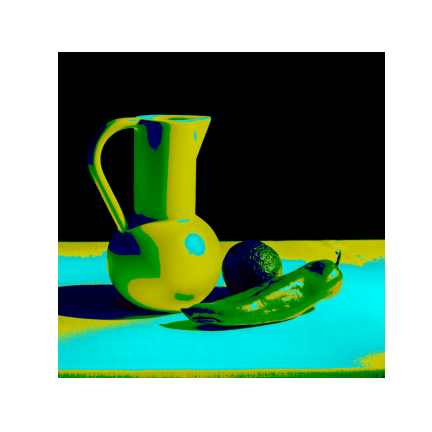
\includegraphics[scale=0.7]{images/colorized_hsv.png}
\caption{Szürkeárnyalatos kép kiszínezése HSV színtérben.}
\label{fig:colorized_hsv}
\end{figure}

A képet a kiszínezés után az egyszerű kirajzolás érdekében visszaalakítottam RGB színterűvé. Jól látható, hogy a két színtérben történő színezés ugyanazt a képet eredményezi.

\Section{Képek színének visszabecslése}

Az előző alfejezetekben bemutatott színezés során a kép színeit általam előre meghatározott színekből, random választottam ki. Ahhoz, hogy valósághűbb színeket tudjunk adni a képeknek, szükséges valamilyen tanító algoritmus használata.  Mivel az én esetben képekről van szó, így kézenfekvő volt, hogy Konvolúciós Neurális Hálót (Convolutional neural networks - CNN) használjak.

A tanító algoritmusok közül a CNN az egyik leghíresebb és legelterjedtebb. Ennek az egyik fő oka, hogy az elődeivel szemben a CNN emberi felülvizsgálat nélkül tudja megtanulni a releváns funkciókat. Széles körben alkalmazzák, például beszédfelismerés, arcfelismerés, számítógépes látás során. A CNN-ek felépítését az emberi és állati agyakban található neuronok ihlették, hasonlóan a hagyományos neurális hálózatokhoz.

A hagyományos, teljesen összekapcsolt (Fully Connected - FC) hálózatokkal ellentétben a CNN a megosztott súlyokat és a lokális kapcsolatokat használja arra, hogy teljes mértékben kihasználja a 2D bemeneti adatstruktúrákat. Mivel ez a művelet kevés paramétert használ, így a képzési folyamat egyszerűbb, emiatt gyorsabb a háló működése.\cite{cnn}

A háló több rétegből épül fel, a leggyakrabban használt rétegeket a következő felsorolás tartalmazza \cite{cnn}:
\begin{itemize}
\item Konvolúciós réteg: A CNN-architektúrában a legjelentősebb komponens a konvolúciós réteg, ami konvolúciós szűrők (ún. kernelek) gyűjteményéből áll. A bemeneti képre ezeket a szűrőket alkalmazza, hogy létrehozza a kimeneti jellemtérképet.
\item Pooling réteg: A pooling réteg fő feladata a jellemtérképek almintavételezése. Más szavakkal a nagy méretű jellemtérképeket összezsugorítja, kisebb térképeket hoz létre, viszont ezzel párhuzamosan a domináns információk többségét megtartja. Néha a CNN teljesítménye ennek a rétegnek az eredményeként csökken, mivel ez a réteg segít a modellnek meghatározni, hogy egy adott funkció elérhető-e az adott bemeneti képen vagy sem.
\item FC réteg: Ez a réteg általában az egyes CNN-architektúrák végén található. Ezen a rétegen belül minden neuron az előző réteg összes neuronjával kapcsolatban áll, ez az úgynevezett Fully Connected megközelítés. A CNN osztályozójaként használják. A bemenete az utolsó pooling vagy konvolúciós rétegből származik, ez a bemenet egy vektor, ami a jellemtérképekből jön létre. Ennek a rétegnek a kimenete a CNN végső kimenete.
\end{itemize}

A CNN általános használati felépítése számos konvolúciós rétegből áll, utána következnek a pooling rétegek, majd a befejező rétegek, amik FC rétegek. A modell bemeneti rétege 3 dimenziós:
\begin{itemize}
\item magasság
\item szélesség
\item mélység
\end{itemize}
Gyakran a magasság és a szélesség megegyezik, a mélység pedig a csatorna számra vonatkozik, például RGB színterű kép esetén a mélység értéke 3.

A konvolúciós réteg pontszorzatot számol a bemenet és a súlyok között. A bemenet a kiindulási képnek egy csökkentett méretű része. Ezután az alrétegek jellemtérképeinek a mintavételezése következik, ami csökkenti a hálózati paramétereket, így a tanulási folyamat felgyorsul. Ezután az összes jellemtérképre alkalmazzák a pooling függvényt, végül az FC rétegek megkapják ezeket a közepes és alacsony szintű jellemzőket, és ezekből magas szintű absztrakciókat hoznak létre. Az osztályozási pontszámokat a befejező réteg segítségével állítják elő, ahol minden pontszám egy adott osztály valószínűségét jelzi. \cite{cnn}

\SubSection{Modell konfigurálása}

A CNN modellemet a \texttt{tensorflow.keras} könyvtár segítségével hoztam létre. A tanításához 11 csendéletet kerestem az \cite{unsplash}. hivatkozásban található oldalon. Az eddig Jupyter munkafüzetben folytatott vizsgálatot a \texttt{program} nevű mappába elkezdtem egy közös programmá implementálni, a CNN modellem is már saját .py fájlban készült. Ebben a \texttt{program} mappában található egy \texttt{images} mappa, ami a tanításhoz használt képeket tartalmazza. A képek nevei a [0, 10] intervallumban található számok.

A modell tanításához létre kellett hoznom a tanító halmazomat. Mivel a textúra alapú K-means algoritmus során ablakokat vágok ki a képről, így kézenfekvő volt, hogy a modellemet is hasonló ablakokkal tanítsam be. Ezért a tanítóhalmaz megalkotásához először kinyerek adott darabszámú ablakot minden egyes képről. Ezeknek az ablakoknak meghatározom a középpontjához tartozó színét, majd átalakítom HSV színterűvé a kapott RGB színt. A HSV szín alapján hozzárendelek egy címkét az adott ablakhoz. A színek felosztását, és a hozzájuk tartozó címkéket az \ref{tab:color_category}. táblázat tartalmazza.

\begin{table}[h]
\centering
\caption{Színek kategorizálása HSV értékek alapján.}
\label{tab:color_category}
\medskip
\begin{tabular}{|c|l|l|l|}
\hline
Címke & Logikai vizsgálat & Szín & RGB kód \\
\hline
0 & $H < 20$ & Vörös & $[255, 0, 0]$ \\
\hline
1 & $H >=20 \, \& \, H < 60$ & Narancssárga & $[255, 165, 0]$ \\
\hline
2 & $H >=60 \, \& \, H < 90$ & Sárga & $[255, 255, 0]$ \\
\hline
3 & $H >=90 \, \& \, H < 120$ & Lime & $[0, 255, 0]$ \\
\hline
4 & $H >=120 \, \& \, H < 150$ & Zöld & $[0, 128, 0]$ \\
\hline
5 & $H >=150 \, \& \, H < 180$ & Akvamarin & $[0, 255, 180]$ \\
\hline
6 & $H >=180 \, \& \, H < 210$ & Cián & $[0, 255, 255]$ \\
\hline
7 & $H >=210 \, \& \, H < 240$ & Világoskék & $[0, 100, 255]$ \\
\hline
8 & $H >=240 \, \& \, H < 270$ & Kék & $[0, 0, 255]$ \\
\hline
9 & $H >=270 \, \& \, H < 300$ & Lila & $[128, 0, 128]$ \\
\hline
10 & $H > 300$ & Magenta & $[255, 0, 255]$ \\
\hline
11 & $V < 0.1$ & Fekete & $[0, 0, 0]$ \\
\hline
12 & $V > 0.9 \, \& \, S < 0.1$ & Fehér & $[255, 255, 255]$\\
\hline
\end{tabular}

\end{table}

Ahol a logikai vizsgálat értéke \texttt{igaz}, azt a címkét fogja megkapni az ablak. Elsőként a fekete és fehér színek vizsgálatát végzem el, mivel ott nem a Hue értékét, hanem a Value és Saturation értékeket vizsgálom. A színeket a már korábban bemutatott \ref{tab:hsv_colors}. táblázat alapján határoztam meg, viszont kibővítettem néhány plusz árnyalattal.

Mielőtt még hozzáadnám az ablakot a tanító halmazomhoz, átalakítom szürkeárnyalatos képpé, hiszen az a célunk, hogy szürkeárnyalatos képekre adja vissza a megfelelő színt.

A tanító halmaz kinyerése után következik a modellem felépítése és betanítása. Ennek az algoritmusa a következő kódrészletben látható.
\begin{python}
def get_model():
    """
    Method for creating the CNN model.
    :return: the created CNN model
    """
    x_train, x_test, y_train, y_test = get_training_data()

    #normalizing the pixel values
    x_train=x_train/255
    x_test=x_test/255

    model=Sequential()

    model.add(Conv2D(64,(3,3),activation='relu',input_shape=(15, 15, 1)))
    model.add(MaxPool2D(2,2))

    model.add(Conv2D(32,(3,3),activation='relu'))
    model.add(MaxPool2D(2,2))

    model.add(Flatten())
    model.add(Dense(32, activation='relu'))

    model.add(Dense(13, activation='softmax'))

    opt = Adam(learning_rate=0.001)

    model.compile(
        loss='categorical_crossentropy',
        optimizer=opt,
        metrics=['accuracy'])

    model.fit(
        x_train,
        y_train,
        epochs=30,
        validation_data=(x_test, y_test))

    return model
\end{python}

Első lépésként meghívom a \texttt{get\_training\_data} nevezetű függvényt, aminek a működését az imént ismertettem. A metódustól válaszként megkapom a tanító és a tesztelő halmazomat. Az ablakok amiket megkapok $15 \times 15$ méretűek. Normalizálom a pixelek értékeit, ami azt jelenti hogy 0 és 1 közötti értékké alakítom őket.

Ezután létrehozok egy szekvenciális modellt, és megadom az első konvolúciós réteget. A kimeneti dimenziónak, vagyis a szűrők számának 64-et adok meg, a kernel mérete $3 \times 3$. A megadott aktivációs függvény \texttt{RELU} típusú ami azt jelenti, hogy az összes bemeneti adatot pozitív számmá alakítja. Az utolsó paraméter a bemeneti adat típusa, ami $15 \times 15 \times 1$, mivel ekkora volt az ablakok mérete, és a 3 dimenzió jelzi hogy ez egy szürkeárnyalatos kép, hiszen csak 1 csatornája van.

Ezután megadok egy pooling réteget aminek a bemeneti paramétere az a méret, amin szeretném hogy a vizsgálatot végezze. Az én esetemben $2 \times 2$ méretű ablakokra fogja a maximumot venni.

Hozzáadom az előző 2 réteget még egyszer annyi különbséggel, hogy a szűrők számát a konvolúciós rétegnél most csak 32-re állítom.

Ezután 2 \texttt{Dense} réteggel megadom a kimeneti adatok formáját. Az első rétegnél a 32 érték következik az utolsó konvolúciós rétegnél megadott értékből. A második \texttt{Dense} rétegnél azt adom meg, hogy hány féle kimenetele lehet a vizsgálatnak. Mivel 13 színre vizsgálok, így 13 féle eredménye lehet. Az aktivációs függvényként megadott \texttt{softmax} azt jelenti, hogy minden lehetőségre generál egy $[0, 1]$ közötti valószínűséget. A tanítás során megadott \texttt{categorical\_crossentropy} ezeknek a valószínűségeknek a segítségével fogja mérni a modell teljesítményét.

A modell építése és ellenőrzése után már csak a tanítás és a tesztelés van hátra.

\SubSection{Tesztelés}

A modell hatékonyságát ábrázoló grafikon az \ref{fig:cnn_accuracy}.ábrán látható.

\begin{figure}[h]
\centering
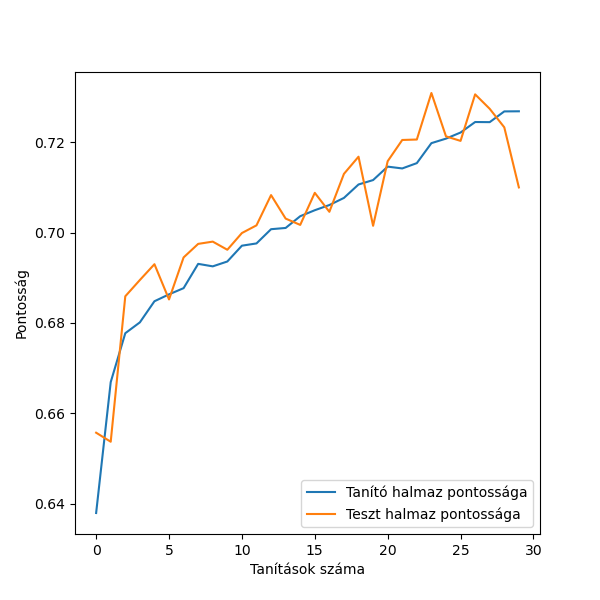
\includegraphics[scale=0.7]{images/cnn_accuracy.png}
\caption{CNN modell pontosságát szemléltető grafikon.}
\label{fig:cnn_accuracy}
\end{figure}

A modell pontosságát maximum 72\%-ra tudtam megnöveli, és sajnos így sem produkál olyan működést, mint amilyet vártam tőle. A modellt próbáltam javítani a képek módosításával, a tanító halmaz növelésével, csökkentésével, az adatok szűrésével, a modell rétegeinek módosításával, de a fentebb látható konfigurációnál nem sikerült jobbat létrehoznom. Az eddigi vizsgálatokat, és a CNN futási eredményeit az \ref{fig:result_all_kmeans}. ábra tartalmazza K-means módszerrel szegmentált képekre, és az \ref{fig:result_all_superpixel}. ábra tartalmazza szuperpixel metódusok segítségével szegmentált képekre.

\begin{figure}[h]
\centering
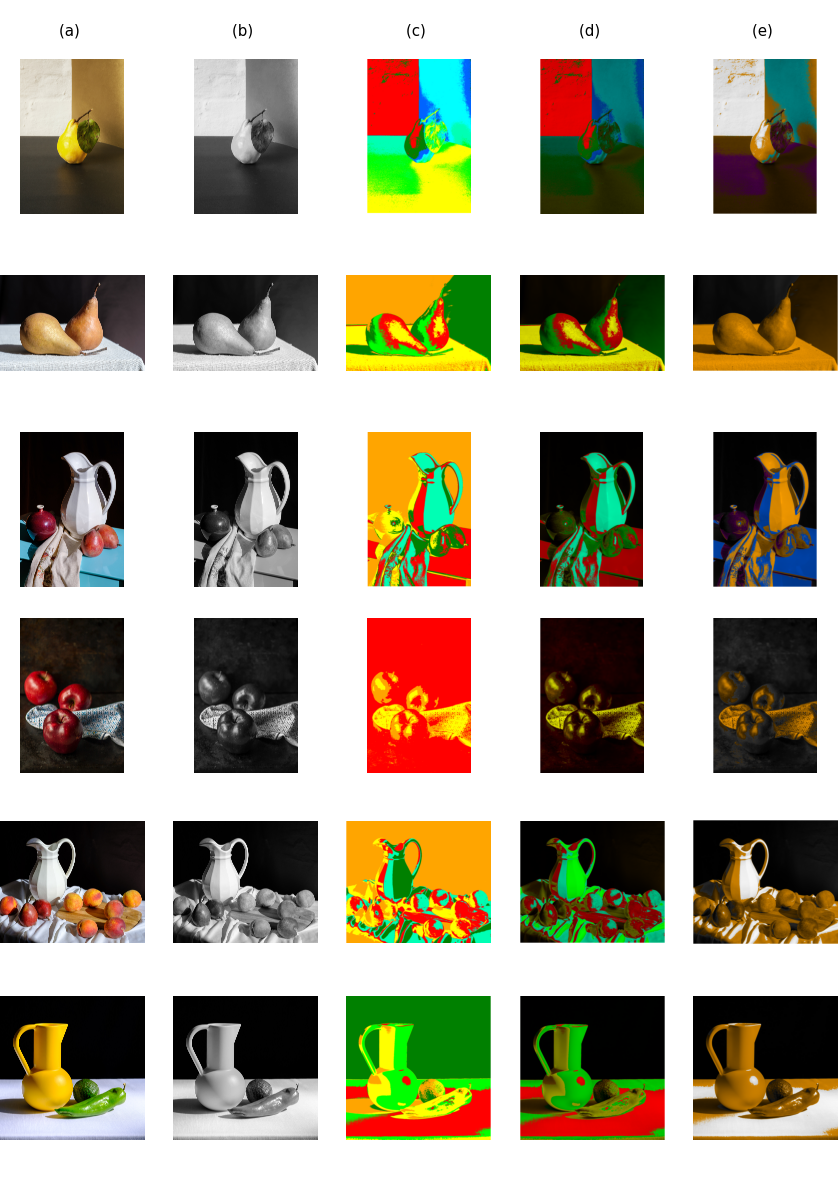
\includegraphics[scale=0.5]{images/result_all_kmeans.png}
\caption{A vizsgálatok futtatása CNN színezéssel az összes K-means módszerrel klaszterezett teszt képre. Az oszlopok a következő képeket tartalmazzák: (a) eredeti, színes kép (b) eredeti, szürkeárnyalatos kép (c) textúra alapú k-means szegmentált kép (d) random színekkel színezett kép HSV színtérben (e) CNN használatával színezett kép HSV színtérben }
\label{fig:result_all_kmeans}
\end{figure}

\begin{figure}[h]
\centering
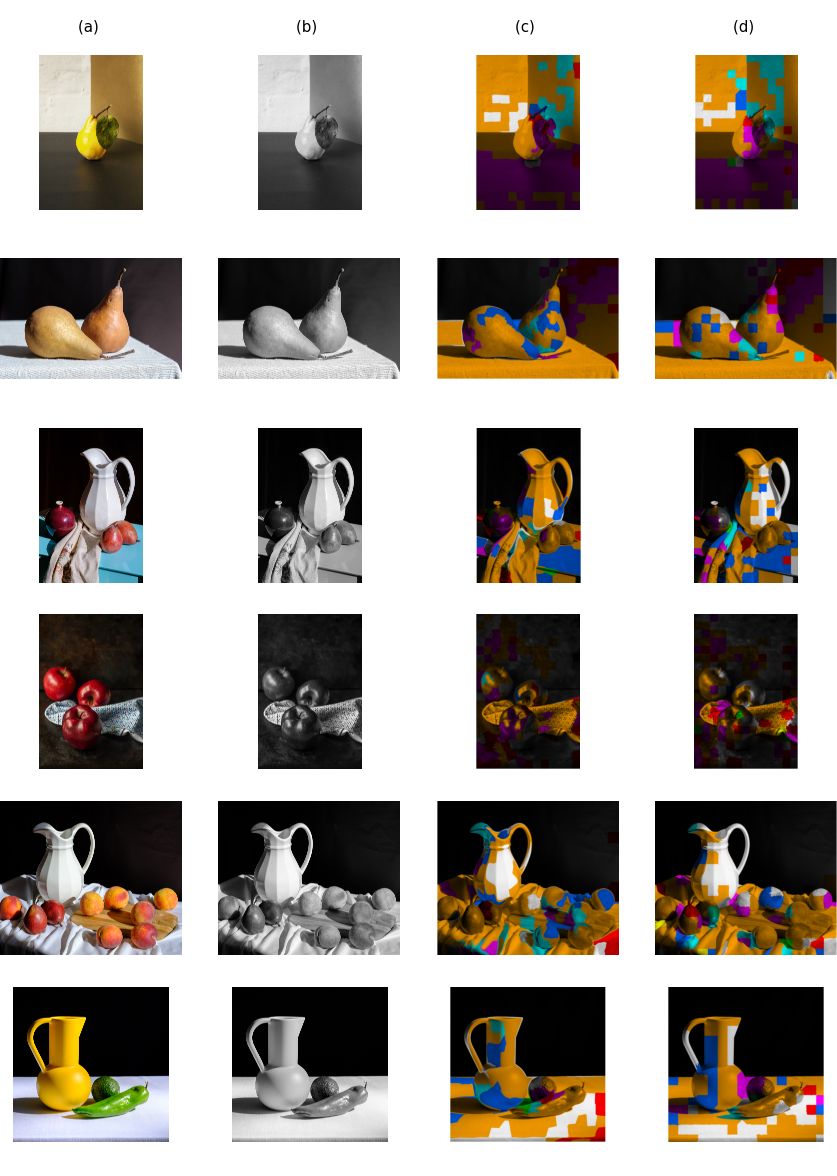
\includegraphics[scale=0.5]{images/result_all_superpixel.png}
\caption{A vizsgálatok futtatása CNN színezéssel az összes Szuperpixel módszerekkel klaszterezett teszt képre. Az oszlopok a következő képeket tartalmazzák: (a) eredeti, színes kép (b) eredeti, szürkeárnyalatos kép (c) SLIC módszerrel szegmentált kép HSV színtérben színezve (d) Watershed módszerrel szegmentált kép HSV színtérben}
\label{fig:result_all_superpixel}
\end{figure}

K-measn esetén adott klaszterhez a szín meghatározása többségi döntés alapján történik, miután kinyertem a minta ablakokat és szegmentáltam őket. Az egy címkét kapott ablakokat átadom a CNN modellemnek, majd a CNN által meghatározott címke számlálóját növelem. Amire a legtöbb szavazat érkezik egy adott címkén belül, az a győztes szín.

A szuperpixel módszerek esetén minden szuperpixelre egy vizsgálatot végzek, és annak a predikciónak az eredménye lesz a kapott szín. Szembetűnő, hogy csak a különböző szuperpixeleket vizsgálva gyakori, hogy az azonos objektumokon belül más-más színeket jósol. Ezt lehetne javítani több mintavétellel az adott szuperpixeleken belül. Az is jól látszik, hogy a SLIC esetén a színezés szebben megvalósult, mint a Watershed esetén. 

Az \ref{fig:result_all_kmeans}. ábrán megfigyelhető, hogy bár például a 2. képen a körtén belül több szegmenst határozott meg a K-means, a CNN mindegyik szegmensnek ugyanazt a színt jósolta, így a körte egy színű lett. Viszont az is látható, hogy ugyan ezt nem tudta megvalósítani az 1. képen.

Ami szembetűnő, hogy a modell sok esetben sárga és fehér színeket jósol az adott ablakokra. Ez abból eredhet, hogy a tanító halmazban több sárga szín található, mint zöld vagy kék, viszont a sárga szín csökkentésével sem értem el jobb eredményt, abban az esetben egy másik színt használt ugyan olyan gyakorisággal. A legtöbbször előforduló szín a minták során a fekete, a színek meghatározásánál viszont a modell nagyon ritkán jósolt fekete színt egy adott klaszterhez. 

